\chapter{Background} \label{chap:background}
In order to conduct the comparison effectively, it is necessary to first lay a good theoretical basis of event-driven architecture, event stream processing and the concrete roles of an \acrshort{esp} platform. Based on that, a comprehensive set of evaluation metrics can be determined.


\section{Event Driven Architecture}
\subsection{Monolithic Architecture}
A monolithic application focuses on the simplicity. All components including user interface, business logic and data accessing services are developed, packaged and deployed in a single unit \cite{monolith}.

Monolithic applications are straightforward to develop and test since the control flow is very transparent. Deployment and scaling are also simple because there is only a single software artifact. A monolithic architecture can also result in better performance for small application with few users \cite{al2018comparative}. Therefore, when starting a new software project, monolith should be the first choice to be considered \cite{monolithfirst}. 

\subsection{Microservices with Event-Driven Approach}
As the application expands, monolithic architecture gradually becomes more rigid and harder to adapt to the agile development cycle. A small change in any service will lead to rebuilding and redeployment of the entire application. Moreover, developers in the team must work closely together and cannot freely establish their own paces. For that reason, the microservices architecture arises. In general, an application is disassembled into services according to different business capabilities \cite{microservicesfowler}. These services are self-contained and loosely-coupled with each other. Each of them maintains a separate database and expose its data with other only via a mutually agreed contract. Since every service itself is an independent deployable, it can have its own development cycle and technology stack. Services also allow finer-grained scaling of the application. This is very useful for reducing cost when deploying the application to the cloud \cite{villamizar2016infrastructure}.

In microservices architecture, services need to have a mechanism to coordinate and work together to achieve end results. There are typically two approaches for this task, namely, request-driven and event-driven \cite{stopford2018designingeventdriven}.

In the first approach, a service sends command to request for state change or queries current state in other services. This method is hard to scale because the control logic concentrates on the sender of requests. Adding a new service usually involves code change in other to include it in the control flow. For the latter approach, services communicate with each other using events.

\textbf{Event}\\
An event is simply a fact stating what has happened in the system. Whenever a service updates its state, it sends out an event. Any other service can listen and operate on this event without the sender knowing about it. This leads to inversion of control where the receiver of events now dictates the operational logic. As a result, services of the system can be more loosely coupled. New service can be easily plugged in the system and start to consume events without the need to modify other services. There are three common ways to use events, namely, event notification, event-carried state transfer and event sourcing \cite{martinfowlereventdriven}.

\textbf{Event Notification}\\
The events are used only for notifying about a state change on the sender. Receiver decides which operation should be executed upon receiving the events. This usually involves querying for more information from either the publisher of events or another service.   
\begin{figure}[h]
	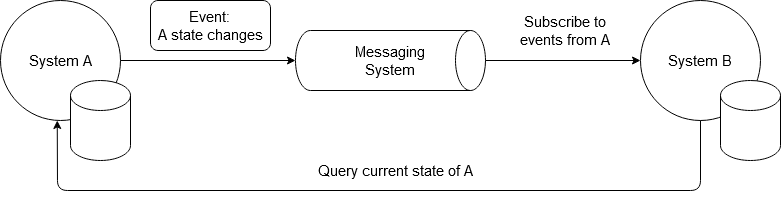
\includegraphics[width=\linewidth]{images/eventnotification.png}
	\caption{Services coordination with event notification.}
	\label{fig:eventnotification}
\end{figure}

The approaches of event notification and request-driven ensure a minimum level of coupling by letting each service manage its own data and only share when being requested. Another advantage is that the state of each service is consistent throughout the entire system since it only exists in one place. Nevertheless, these approaches only works at their best when services are truly independent from each other which is usually not the case in reality. It is unavoidable that services must maintain a certain level of dependency and sharing of data. When services grow with more functionalities, they need to expand the service contract to expose more data to outside which then leads to higher coupling. This is known as the dichotomy of data and services \cite{stopford2018designing}. Therefore, the two following patterns tackle this problem by actively allowing services to openly share their data instead of encapsulating it within each service.

\textbf{Event-Carried State Transfer}\\
With this pattern, each event encloses more detail information about what has been changed as well as the new value. As a result, current state of any service can be reconstructed anywhere by applying its published events on the same initial state in the same order. Therefore, every subscriber can retain a local state replica and keep it synchronized with the source of events.

\begin{figure}[h]
	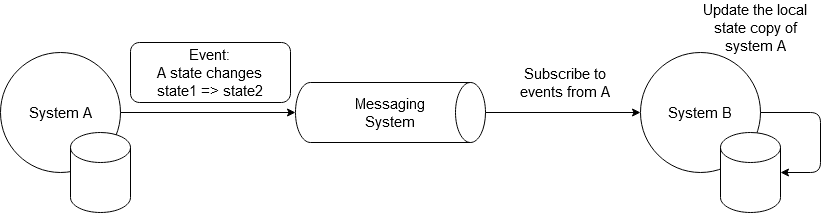
\includegraphics[width=\linewidth]{images/eventstatetransfer.png}
	\caption{Services coordination with event-carried state transfer.}
	\label{fig:eventstatetransfer}
\end{figure}

When a service keeps a state copy of another locally, it can access this data faster and becomes independent of the online status of the source of data. Nevertheless, having multiple copies of data across the system also means that the system can be in inconsistent state temporarily or even worse permanently if it is not designed carefully. This concern is closely related to the problem of how to atomically update the local state and publish a corresponding event \cite{eventstatetransferproblem}.
%Therefore, care should be taken when applying event-driven architecture to not overcomplicate the system.

\textbf{Event Sourcing and \acrfull{cqrs}}\\
 


\section{Event Stream Processing} \label{section:eventstreamprocessing}
With the increasing amount of data, the demand about how data is processed and analyzed also evolves over time. In the early day, data is usually collected over a period of time and stored in a big bounded batch in a data warehouse. Some scheduled batch jobs will then go over the entire batch of data to generate insights and reports tying to the needs of the organization. However, this type of data processing gradually cannot keep up with the need of faster analysis allowing companies to response more timely to change. Therefore, the concept of stream processing begins to emerge.


Unlike its batch counterpart, stream processing aims at handling unbounded data which is a better form for representing the flow of events in real world given their continuous and boundless nature. By processing this influx of data continuously as they arrives, events and patterns can be detected with low latency making stream processing more suitable for real-time use cases. Moreover, the input data can come from an uncountable number of sources with varying transmission rates. Therefore, data may arrive late and out of order with respect to the time it is generated at the source. In this case, for it sees data in an endless fashion, stream processing gives more tolerance for late data and more flexibility to assemble data into windows and sessions to extract more useful information. It is even suggested that a well-designed stream processing system with guarantee of correctness and the capability to effectively manage the time semantics could surpass batch processing system \cite{stream101}. Back in the time when using stream processing was a trade-off between accuracy and low-latency, it was a popular idea to run two batch and stream processing pipelines in parallel to achieve both fast and correct results \cite{lambdaarchitecture}.  As stream processing engines grow more mature and accurate, the demand for such system is lessened \cite{questionlambdaarchitecture}.
\subsection{Stream Processing and Event-Driven Architecture}

Moreover, stream processing is not merely a data processing paradigm to achieve low latency result. Applying the concept of streaming on the architectural level in event-driven systems also has the potential to help build more scalable and resilient applications. The problem of coupling emerges not only between services of applications but also between data systems in general. A sophisticated software system can comprise of multiple data systems with different functionalities such as relational database, document store, cache, monitoring system, data warehouse. Data needs to be shared and synchronized between these components in an efficient way. This can quickly turns the entire system into a big tangled mesh. As an example, this problem was experienced at LinkedIn as their system became increasingly complex \cite{eventstreamingplatform}. 

\begin{figure}[h]
	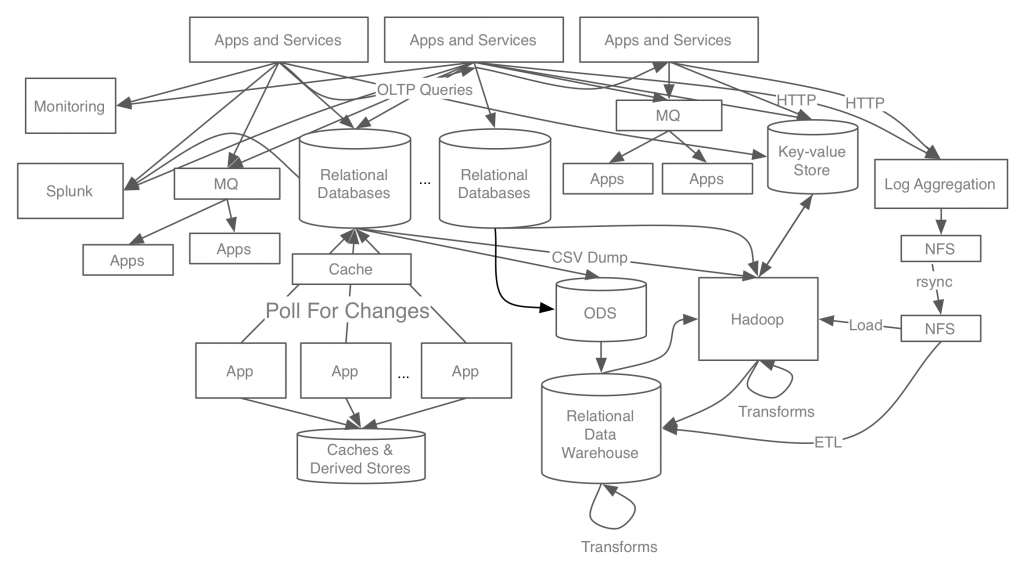
\includegraphics[width=\linewidth]{images/linkedin-data-flow-ugly.png}
	\caption{The tangled data systems at LinkedIn in the old day \cite{eventstreamingplatform}.}
	\label{fig:tangledsystem}
\end{figure}

This problem can be tackled by using stream processing in event-driven systems. In such systems, every operation, state change or any information can be recorded in form of an event. Events from all services are gathered and written orderly to an append-only log called event stream. On the contrary to the previous approach where data is encapsulated in each service, this stream is used as the single source of truth shared by all services. Any data service in the system can consume and process this log of raw events using stream processing to generate a local replication of the current system state. This log-centric design fits seamlessly into a distributed environment with numerous moving components to allow data to be replicated among services with minimal coupling \cite{logjaykreps}. Moreover, services also have the flexibility to derive different data structures from the raw events to match their specific access pattern. The task of data representation is now done at individual data service instead of in the central data store. This is referred by Martin Kleppmann as turning the database inside out \cite{kleppmann2016making}. The result is a more neatly organized system with every services synchronize and communicate via the event streams.

\begin{figure}[h]
	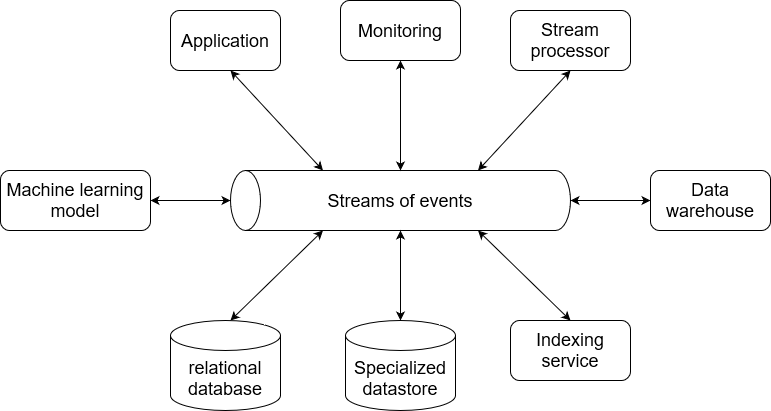
\includegraphics[width=\linewidth,height=7cm]{images/eventstreamprocessing.png}
	\caption{System with streams of events as the single source of truth.}
	\label{fig:eventstreamprocessingsystem}
\end{figure}

\section{\acrlong{esp} Platform}
An \acrshort{esp} platform must facilitate the construction of software systems revolving around streams of events. Therefore, it must have a number of fundamental capabilities. Firstly, it must provide the mechanism for events storage. Optimally, it should also support the option to persist events for an infinite period of time since this will be the single source of truth that the entire system depends on. Accessing interface must be provided for applications to publish and consume events. The platform should also enable the processing on the events streams either by providing a native stream processing tool or integrating with external stream processing framework. Moreover, the platform should come with ready-to-be-used tools to integrate with a wide range of existing data systems effortlessly including also legacy systems.

The order of events must be preserved by the platform throughout their entire life cycle: in storage, transit and under process. All of these capabilities should be in a real-time, high throughput, scalable and highly reliable fashion so that the platform would not become the bottleneck in the system. Finally, the platform must have a rich set of utility tools for monitoring and management.



